\documentclass{article}


\usepackage{arxiv}

\usepackage[utf8]{inputenc} % allow utf-8 input
\usepackage[T1]{fontenc}    % use 8-bit T1 fonts
\usepackage{hyperref}       % hyperlinks
\usepackage{url}            % simple URL typesetting
\usepackage{booktabs}       % professional-quality tables
\usepackage{amsfonts}       % blackboard math symbols
\usepackage{nicefrac}       % compact symbols for 1/2, etc.
\usepackage{microtype}      % microtypography
\usepackage{graphicx}       % define the path of figures
\graphicspath{ {./img/} }
\usepackage{setspace}       % set the space between lines
\doublespacing

\title{Report\\Self-drive car rental\\ \large{COMP7320 - Professional Methodologies for Information Systems}}


\author{
    Kaiyu Lin\\
    Department of Computer Science\\
    Hong Kong Baptist University\\
    \texttt{18438342@life.hkbu.edu.hk}
    \And
    Matteo Azzarelli\\
    Department of Computer Science\\
    Hong Kong Baptist University\\
    \texttt{18432468@life.hkbu.edu.hk}
    \And
    Nurzhan Izdauov\\
    Department of Computer Science\\
    Hong Kong Baptist University\\
    \texttt{18446388@life.hkbu.edu.hk}
    \And
    Rongjia Weng\\
    Department of Computer Science\\
    Hong Kong Baptist University\\
    \texttt{18438512@life.hkbu.edu.hk}
    \And
    Saurabh Kumar\\
    Department of Computer Science\\
    Hong Kong Baptist University\\
    \texttt{18441238@life.hkbu.edu.hk}
    \And
    Sheetal Pargain\\
    Department of Computer Science\\
    Hong Kong Baptist University\\
    \texttt{18430481@life.hkbu.edu.hk}
%   %% examples of more authors
%   \And
%  Elias D.~Striatum \\
%   Department of Electrical Engineering\\
%   Mount-Sheikh University\\
%   Santa Narimana, Levand \\
%   \texttt{stariate@ee.mount-sheikh.edu} \\
  %% \AND
  %% Coauthor \\
  %% Affiliation \\
  %% Address \\
  %% \texttt{email} \\
  %% \And
  %% Coauthor \\
  %% Affiliation \\
  %% Address \\
  %% \texttt{email} \\
  %% \And
  %% Coauthor \\
  %% Affiliation \\
  %% Address \\
  %% \texttt{email} \\
}

\begin{document}

\maketitle

\newpage

% \begin{abstract}
%     In this report we are going to review the main concepts expressed by Mr. Edmon Chung in the talk held the day 29 January 2019.
%     The main point is the Global Internet Governance and some of the related concepts: like copyright, privacy, security and anonymity. Obviously these arguments involve also the policy of stats and we can see how some of them manage these arguments, with some restrictions, and in particular we could understand why privacy and security are in contradiction.
% \end{abstract}


% keywords can be removed
%\keywords{Global Internet Governance \and Privacy \and Security \and Anonymity}


\section{Executive summary}
    In this document we have presented the detailed deliverables that describe the system development plan of our proposed system that is an information system that will provide its customers a platform to rent cars online seamlessly. This Self-drive car rental system is an initiative to tackle problems such as environment sustainability and faster renting of cars without the need of a middle-man or agency. The system we proposed can be used across multiple platforms such as mobile and website. In order to understand if the system implementation is justifiable we have done a thorough feasibility analysis to show the pros of accepting this system. Also, our system requirements focus on what functions the system should provide to both its users and admin and what requirements it should have in order to be successful. Through our system diagrams such as data flow diagrams and use case diagrams we represent the main functions of our systems such as car rental and registration in a visual way. We are highly hopeful that through the successful development and implementation of this system, the world will be a better place for you and us.
    
\section{Problem scenario/System request}
    \subsection{System request}
        \subsubsection{Business Need:}
        \begin{itemize}
            \item To develop a car sharing system in order to achieve greater environmental sustainability by making cars more affordable in Hong Kong without increasing their number.
            \item To make the whole process much easier and faster by affording both cross-platform mobile and web application.
        \end{itemize}
        
        \subsubsection{Functionality:}
        \begin{itemize}
            \item Immediate booking of available cars using either mobile phone or website.
            \item Online and fast payment with linking a credit card to the system.
            \item Avoid any inconvenience with the parking issues using company’s parking facilities.
        \end{itemize}
        
        \subsubsection{Expected Value:}
        \begin{itemize}
            \item Tangible:
                \begin{itemize}
                    \item 1,000,000USD revenue in the first year.
                    \item 580,000USD net profit from the sales of the first year.
                \end{itemize}
            \item Intangible:
                \begin{itemize}
                    \item Increasing customer service of car sharing services.
                    \item Achieving greater environmental sustainability.
                    \item Reducing the number of private cars to decrease the number of traffic jam issues.
                \end{itemize}
        \end{itemize}
        
        \subsubsection{Special Issues or Constraints:}
        \begin{itemize}
            \item The website must be launched after 3 months.
            \item The mobile applications for both Android and iOS platforms must be in place within the next 4 months.
            \item The parking facilities should be arranged no later than the launch of the website. 
        \end{itemize}
        
        \newpage
\section{Feasibility analysis}
    \subsection{Market Demand Analysis}
    
    In Hong Kong, although there is no need to pay customs duties when buying a car, the average number of car owners in the local area is much worse than other big cities.
    According to statistics, the number of people with a driver's license is close to 1.7 million, while the number of private cars is 600,000 , which means that 1.1 million people are “car-free”, and the market demand is considerable.
    
    Meanwhile, according to research, users are more inclined to travel 10-30 kilometres, which is one of the most important use scenarios for rental cars.
    Rental cars can meet the needs of car-free family short-distance travel privacy and flexibility, and are favoured by users.
    
    \subsection{Technical Analysis}
    
    In fact, the shared car system is essentially a platform for information docking.
    Users use this platform to query and use cars.
    Currently, many similar types of software use similar systems, such as OfO,Mobike,Airbnb, whose functional requirements are not complicated.
    
    However, this system still faces several challenges.
    First of all, in a place where the signal is not good, if the system is unable to connect to the network or malfunction when the user is driving the car, whether the system can continue to support the service shared by the car.
    Secondly, how to detect whether a car needs to be repaired is also a problem.
    Manual inspection and maintenance will increase costs.

    \subsection{Economic Analysis}
    
    Due to the heavy capital attribute of the automobile, the initial input cost of the industry is relatively high, so the intervention of capital is more needed, which increases the difficulty.
    
    In addition, the daily operating costs are also more complicated: parking space costs, fuelling costs, accident costs, vehicle maintenance and repair costs.
    Costs incurred by consumers themselves: violations, accidents, etc.
    
    Of course, these costs must theoretically be borne by consumers themselves, but this will greatly affect the consumer experience, so the operators must pay attention to the communication work here.
    
    \subsection{Operational Analysis}
    
    There are many links involved in the process of using sharing cars, such as: vehicle scheduling, parking management, fuelling management, insurance claims, road rescue, cleaning services, etc.
    Every links would impact the whole system operation seriously.
    
    \subsection{Legal and Contractual Analysis}
    
    There are three main legal and contractual risks related to the car-sharing systems.
    The first one is that there is no enough space for sharing-car parking.
    It would make user parking illegally if they could not find the suitable place.
    It would receive punishment from the relevant agencies.
    
    Meanwhile,the license resources for new vehicles are certain scarce resources, and Hong Kong also has quantitative control.
    So,license resources are considered as a very important constraint.
    
    Furthermore,in the process of using the vehicle, problems such as untimely handling of violations and influencing the use of internal health are often encountered, which increases the burden on vehicle management.

    
\section{System requirements}
    \subsection{Functional requirements}
        \textbf{User}
            \begin{itemize}
                \item User should be able to register an account in the app to rent a car.
                \item User should be able to delete the account.
                \item Users should be able to login to their account.
                \item Users must be able to browse through all the cars in the catalog.
                \item Users should be able to view the details of a specific car.
                \item Users must be able to rent a car based on hours or days.
                \item Users must be able to cancel the reservation they made earlier.
                \item Users must be able to edit the reservation they made.
                \item Users must be able to search for vehicles using filters such as lowest price, most popular, seat capacity and distance.
            \end{itemize}
        \textbf{Admin}
            \begin{itemize}
                \item The admin must be able to register new cars through the system.
                \item The admin must be able to remove any car from the system
                \item The admin must have access to view the reservations made.
                \item The admin must be allowed to edit the information of each car or model.
            \end{itemize}
        \textbf{System}
            \begin{itemize}
                \item The system must be able to verify the driver license of the user.
                \item The system must be able to get the current location of the user.
                \item The system should be able to display the nearest cars and drop-off points respective to each user based on their current location.
                \item The system should calculate the rental fee based on model and duration.
                \item The system must generate a QR code once a car booking is successfully made.
                \item The system must be able to keep track of the GPS location of each car.
            \end{itemize}
    \subsection{Nonfunctional requirements}
        \textbf{Performance Requirements}
            \begin{itemize}
                \item System should be able to maintain high amount of users in the same time without crashing.
                \item Exchange of data and performance speed should be high without lagging.
                \item System should be able to show any available offers and customers should be able to do payment without entering the information every-time.
                \item System should recover from anything if goes wrong.
                \item It should display correct and relevant information in all devices(multiple-platforms).
                \item System should notify the users of all the activities performed through email or text message.
            \end{itemize}
        \textbf{Security Requirements}
            \begin{itemize}
                \item All the transmission between user and the system should be highly secured.
                \item System should be able to prevent from any threat.	
                \item Verifying security certificates for website.
                \item Should able to identify illegal payment methods being used.
                \item Should able to check the authentication of the input data from users,like false email address.
            \end{itemize}
        \textbf{Quality Attributes}
            \begin{itemize}
                \item User friendly environment with visually appealing system should be maintained.
                \item Easy to use and see navigation.
                \item Contents should be easy to readable.
                \item Some part of the system functionality should be available for the not logged in users like searching for the cars models , car rental prices and policies etc.
            \end{itemize}

    
\section{Level-0 DFD of the system}
In Fig.~\ref{fig:Level0DFD} is shown the level-0 DFD of our system.
    \begin{figure}[h]
        \centering
        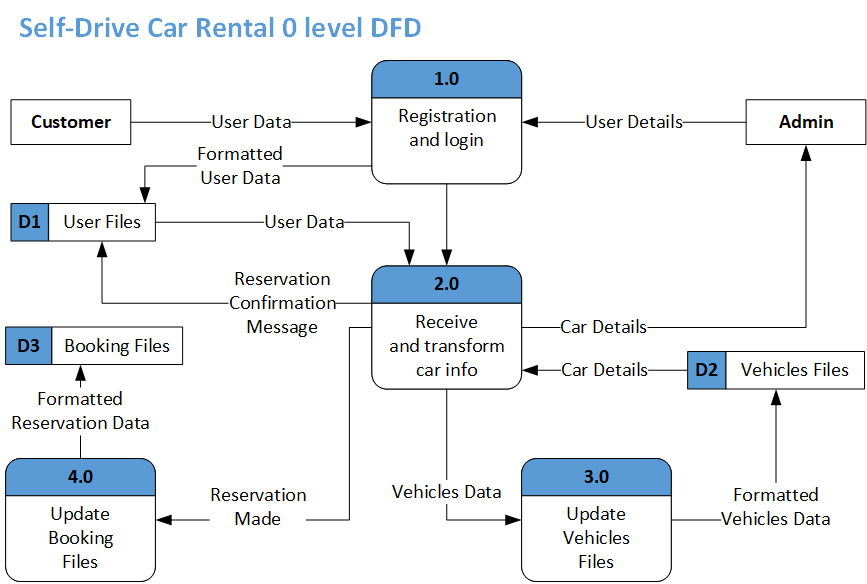
\includegraphics[width=\textwidth]{img/Level0DFD.png}
        \caption{Self-Drive Car Rental 0 level DFD.}
        \label{fig:Level0DFD}
    \end{figure}

\section{Object Oriented (OO) Analysis and Design}
    \subsection{System description}
    
    \textbf{System overview}
    \begin{itemize}
        \item This car-sharing system is suitable for everyone living in Hong Kong or visiting this region as a tourist. Because the main mission of it is to provide affordable car rental for them and make life easier for everyone.
        \item Self-drive car rental has three main subsystems, as finding a car, booking and returning it. All of these functionalities are obviously related to each other in order to provide very reliable and completely automated cross-platform mobile and web application.
    \end{itemize}
    
    \newpage
    \textbf{System functionality}\\
    As we mentioned before, there are three main functions of an application.
    \begin{itemize}
        \item Finding a car - a functionality used to locate the closest and available car to choose the most convenient and appropriate one.
        \item Booking a car - a functionality used to book a car for a certain time-slot in which it is going to be used by a client.
        \item Returning a car - a functionality used to return a car which was previously found and booked, in order to complete the whole process.
    \end{itemize}
    
    \textbf{Components}
    \begin{itemize}
        \item Online Web application will contain all the functionalities of the system. The users will be able to find, book and return a car using this platform. The only exception is that it will not be able to help the users to open/close a car.
        \item Mobile platforms for both Android and iOS will be mostly used to unlock the door of the booked car because you will need to scan the QR code on the machine to unlock it. It can be also used to other services as finding, booking and returning.
    \end{itemize}
    
    
    \subsection{Use Case Diagram}
        \begin{figure}[h]
            \centering
            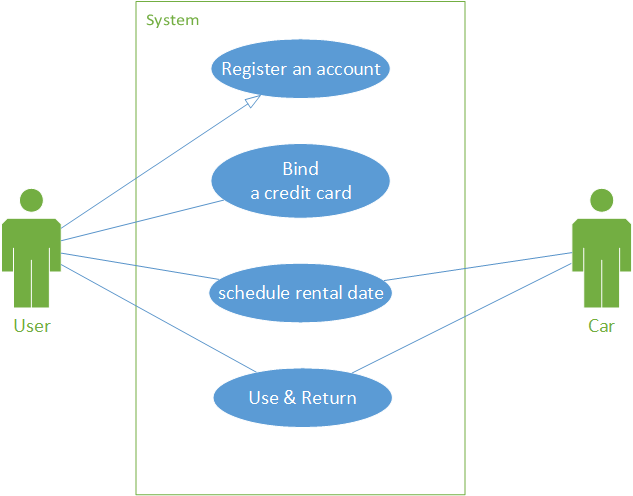
\includegraphics[width=0.6\textwidth]{img/UseCaseDiagram.png}
            \caption{The use case diagram.}
            \label{fig:useCaseDiagram}
        \end{figure}
    
    \newpage
    \subsection{Class Diagram}
        \begin{figure}[h]
            \centering
            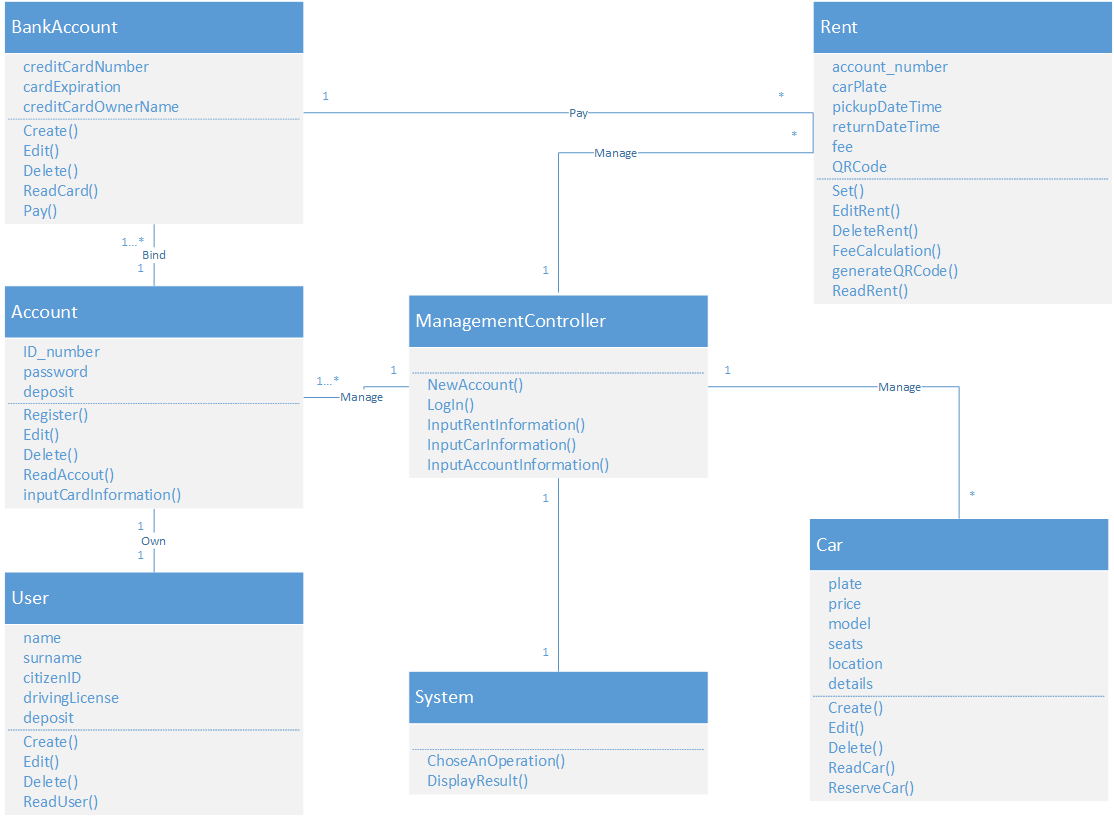
\includegraphics[width=0.8\textwidth]{img/ClassDiagram.png}
            \caption{The class diagram.}
            \label{fig:classDiagram}
        \end{figure}
    \newpage
    \subsection{Sequence Diagrams}
        \begin{figure}[h]
            \centering
            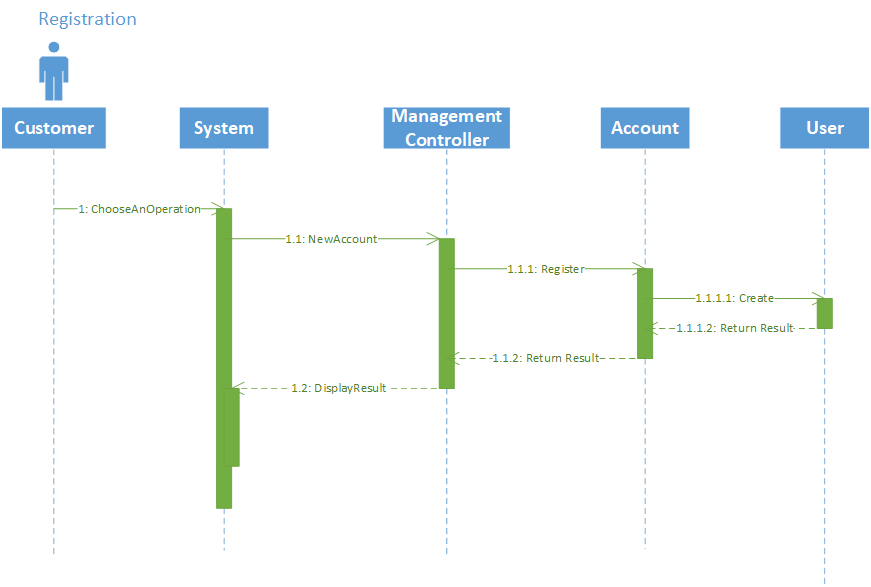
\includegraphics[width=0.75\textwidth]{img/SequenceDiagramRegistration.png}
            \caption{Registration Sequence Diagram.}
            \label{fig:sequenceDiagramRegistration}
        \end{figure}
        
        \begin{figure}[h]
            \centering
            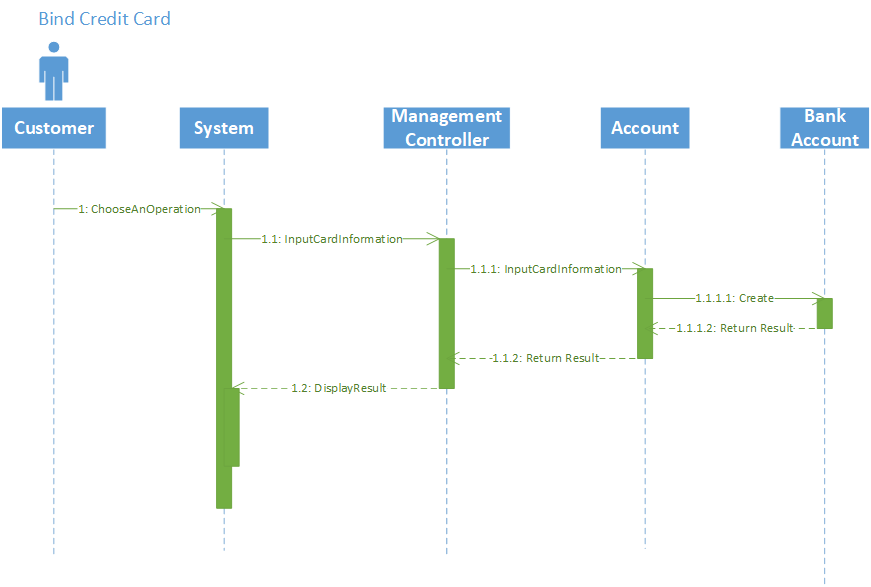
\includegraphics[width=0.75\textwidth]{img/SequenceDiagramBindCard.png}
            \caption{Bind a Card Sequence Diagram.}
            \label{fig:SequenceDiagramBindCard}
        \end{figure}
            
        \begin{figure}[h]
            \centering
            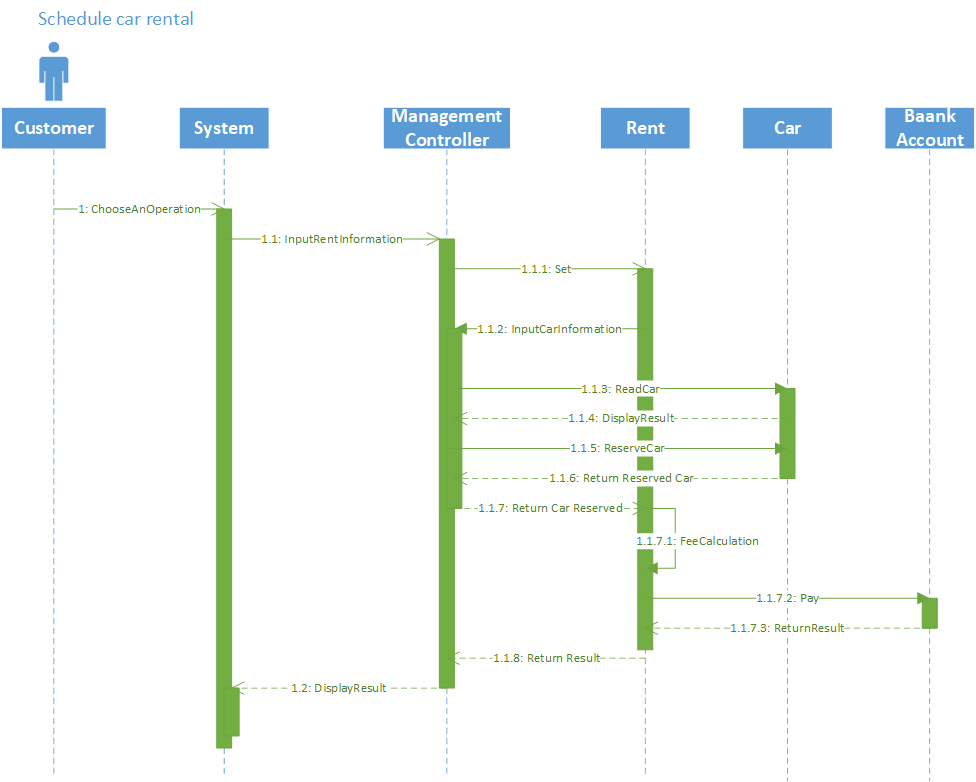
\includegraphics[width=0.75\textwidth]{img/SequenceDiagramRentCar.png}
            \caption{Rent a Car Sequence Diagram.}
            \label{fig:SequenceDiagramRentCar}
        \end{figure}

%\bibliographystyle{IEEEtran}  
%\bibliography{references}

\end{document}
